%! TEX rootmain.tex

\chapter{Woodwind Instruments}

Woodwind instruments couple a pressure-controlled reed to a resonator whose effective length is adjusted by opening and closing finger holes. The chapter first introduces the bore profiles that best preserve a consistent modal structure under length reduction, then discusses the acoustic role of finger holes and the practical consequences for tuning, temperament, and temperature dependence. Methods for input-impedance computation and for sound radiation are subsequently outlined, and the chapter closes with an overview of common woodwind families, with specific remarks on clarinet, oboe, and saxophone. 

\section{Bore Shapes}

\subsection{Bore Shapes with Finger Holes}

In brass-type instruments nearly the entire horn length, including the flaring bell, is always used as a resonator. For instruments with finger holes the situation is different, because the lower part of the resonator can be partly decoupled by open holes. In this sense, open holes modify the effective acoustic length of the resonator. To preserve a consistent tone quality while the acoustic length is reduced, the resonator should scale as its length changes. A profile that preserves its shape under truncation is described by the power law
\[
S(x) = ax^{\epsilon}
\]
defined for
\[
0 \le x \le L
\]
so that the resonant frequencies \( \omega_n \) scale inversely with the length \( L \). 

\subsection{Power-Law Profiles and Bessel Horns}

For a Bessel horn with parameter \( \epsilon \ge 0 \) extending to \( x = 0 \), the acoustic pressure can be written as
\[
p(x) = Ax^{(1-\epsilon)/2}J_{-(1-\epsilon)/2}(kx)
\]
where \( J_{\nu} \) is a Bessel function of order \( \nu \) and
\[
k = \frac{\omega}{c}
\]
Assuming the bore is essentially open at \( x = L \) and neglecting radiation impedance (ideal open-end condition; radiation reactance can be included via an end correction, and radiation losses affect resonance widths), the normal modes occur at angular frequencies \( \omega_n \) given by the roots of
\[
J_{-(1-\epsilon)/2}\left(\frac{\omega L}{c}\right) = 0
\]
This shows that, when \( \epsilon > 0 \), the mode frequencies \( \omega_n \) scale inversely with \( L \), and that no other horn shape has this property. 

\subsection{Musically Useful Bore Profiles}

The mode frequencies derived from the Bessel condition correspond to input-impedance maxima at the mouthpiece, consistent with driving by a pressure-controlled reed. Based on the root structure of Bessel functions, three candidates are highlighted as musically useful approximations:

\begin{itemize}
    \item \( \epsilon = 0 \) (cylindrical bore), associated with an odd-harmonic series \( 1,3,5,\ldots \)
    \item \( \epsilon = 2 \) (conical bore), associated with a complete harmonic series \( 1,2,3,\ldots \)
    \item \( \epsilon \) slightly larger than \( 7 \), yielding a series close to \( 1,(1!),2,(2!),3,\ldots \), though the large flare rate raises practical difficulties
\end{itemize}

As a consequence, useful bore profiles for reed- or lip-driven instruments using finger holes should approximate cylinders or cones fairly closely. In lip-driven instruments with finger holes (e.g. cornet, serpent), the bore is conical, which supports a complete harmonic series and a true fundamental. Reed-driven woodwinds can be either cylindrical or conical.

\subsection{Input Impedance Review: Cylinder and Cone}

For a cylindrical tube of length \( L \) and cross-sectional area \( S = \pi a^2 \), open at its far end, the input impedance can be approximated as
\[
Z_{\mathrm{in}} \approx jZ_{0}\tan(kL')
\qquad
Z_{0} = \frac{\rho c}{S}
\qquad
L' = L + 0.6a
\]
with impedance maxima at
\[
\omega_n = \left(n - \frac{1}{2}\right)\frac{\pi c}{L'}
\]
For a cone of geometrical length \( L \), with throat area \( S_1 \) at a distance \( x_1 \) from the conical vertex and open at the mouth, the input impedance can be written as
\[
Z_{\mathrm{in}} \approx
jZ_{1}\frac{\sin(kL')}{\sin(k\theta_{1})\sin(k(L' + \theta_{1}))}
\qquad
Z_{1} = \frac{\rho c}{S_{1}}
\]
with
\[
k\theta_{1} = \tan^{-1}(kx_{1})
\qquad
L' = L + 0.6a
\]
Under the hypotheses \( x_{1} \ll L \) and \( \theta_{1} \approx x_{1} \), the modal frequencies become
\[
\omega_n = \frac{n\pi c}{L' + x_{1}}
\]
forming a complete harmonic series. 

\subsection{Cylindrical Versus Conical Bores}

To obtain harmonic behavior, woodwind bores must be close to conical (\( \epsilon = 2 \)) or cylindrical (\( \epsilon = 0 \)). For a cylindrical instrument,
\[
\omega_n = \left(n - \frac{1}{2}\right)\frac{\pi c}{L'}
\]
so the resonance series follows odd harmonics. For a conical instrument,
\[
\omega_n = \frac{n\pi c}{L' + x_{1}}
\]
so the resonance series is fully harmonic. For the same geometrical length \( L \), the fundamental frequency of a cylindrical instrument is about half that of a conical instrument. Typical conical bass instruments (e.g. bassoons) therefore use long pipes, often folded to remain practical in size. 

\begin{table}[!htb]
\centering
\begin{tabular}{lcccccc}
\hline
Instrument  & Musical Range     & Tube Length   & Top Diameter  & Bell Diameter             & Semi-Angle        \\
\hline
Clarinet    & D3--G6            & 664           & 14            & \(16 \rightarrow 60\)     & \(0^{\circ}\)     \\
Oboe        & B\(\flat\)3--G6   & 644           & 3             & \(13 \rightarrow 37\)     & \(0.7^{\circ}\)   \\
Bassoon     & B\(\flat\)1--C5   & 2560          & 4             & 40                        & \(0.4^{\circ}\)   \\
Alto Sax    & D3--A6            & 1062          & 12            & \(70 \rightarrow 123\)    & \(1.6^{\circ}\)   \\
\hline
\end{tabular}
\caption{Representative Bore Dimensions Of Common Woodwinds (Dimensions In Millimetres)}
\end{table}

\section{Finger Holes}

Finger holes change the effective length of the air column, enabling the production of different notes. Early instruments were typically limited to fixed 7-note or 5-note scales, with a small number of holes of simple geometry. Modern instruments support chromatic and extended scales, and use key mechanisms to operate combinations of holes reliably. 

\subsection{Tone Control Through Finger Holes}

Consider a cylindrical tube with one finger hole at a small distance \( D \) from the open end. The open hole has a chimney of height \( l \). The analysis assumes that both \( l \) and \( D \) are small with respect to the wavelength. For a cylindrical pipe of acoustic length \( L' \), the input impedance can be written as
\[
Z = jZ_0 \tan(kL')
\qquad
Z_0 = \frac{\rho c}{S}
\]
where the acoustic length includes the standard open-end correction
\[
L' \approx L + 0.6a
\]
with \( a \) the pipe radius. When the hole is open, the portion of tube from the hole to the open end modifies the overall impedance as if there were an effective change in length. At the position of the hole, the admittance presented to the upstream pipe is the parallel combination
\[
Y = Y_{\mathrm{hole}} + Y_{\mathrm{pipe}}
= -j\frac{S_1}{\rho c}\cot(kl) - j\frac{S}{\rho c}\cot\left(k(D+\Delta)\right)
\]
where \( S_1 \) is the hole cross-sectional area and \( \Delta \) is the end correction at the open end of the main pipe. If \( l \) and \( D \) are small compared to the wavelength, using the first-order approximation \( \cot(x) \approx 1/x \) gives
\[
Y \approx -\frac{j}{\rho\omega}
\left(
\frac{S_1}{l} + \frac{S}{D+\Delta}
\right)
\]
which can be equivalently expressed as
\[
Z \approx j\rho\omega
\left[
\frac{l(D+\Delta)}{S_1(D+\Delta) + Sl}
\right]
\]
A simple continuation of the acoustic tube past the hole position by an amount \( \Delta' \) would present an impedance
\[
Z \approx \frac{j\rho\omega \Delta'}{S}
\]
so that the effective end correction at the hole position is
\[
\Delta' \approx \frac{Sl(D+\Delta)}{S_1(D+\Delta) + Sl}
\]
The acoustic length of the tube with its open hole is therefore reduced below that of the original tube by
\[
\delta = D + \Delta - \Delta'
= \frac{S_1(D+\Delta)^2}{S_1(D+\Delta) + Sl}
\]
In the special case \( S_1 = S \) and \( l \approx \Delta \), the reduction becomes approximately
\[
\delta \approx D + \frac{\Delta^2}{D + 2\Delta}
\]

\paragraph{Considerations} For smaller finger holes, the acoustic-length reduction is considerably less than \( D \). A reduction in \( S_1 \) can be compensated by increasing the distance \( D \) from the open end, implying greater separation between adjacent holes. At higher frequencies, when \( D \) is no longer small compared to the wavelength, the preceding low-frequency approximations no longer hold.

\subsection{Finger Holes Positioning in the Lower Register}

In the lower register of a cylindrical wind instrument, a practical guideline is:

\begin{enumerate}
    \item Start from the hole farthest from the mouthpiece (the instrument foot).
    \item Choose \( S_1 \) and \( D \) so that the pipe undergoes an acoustic-length decrease of \( \SI{12}{\percent} \) (whole tone) or \( \SI{6}{\percent} \) (semitone).
    \item Repeat the same procedure starting from the new acoustic length for the next hole, and so on.
\end{enumerate}

In real instruments, hole placement is more complicated, and must also account for deviations from ideal harmonic relationships caused by the holes themselves, together with constraints on playing comfort.

\subsection{Fingering Systems}

Most wind instruments adopt a fingering system based on a preset configuration. The left hand is placed close to the mouthpiece, and the left thumb supports the instrument from below. Three fingers (excluding thumb and little finger) are used to operate the main finger holes, while other fingers manipulate keys for register changes or for accessing very low or very high notes. The left- and right-hand configuration determines the note produced, and real systems refine this baseline by adding holes and keys that extend the playable range.

\section{Tuning, Temperament, Temperature}

\subsection{Reference Pitch}

A practical reference for orchestral tuning is the standard pitch
\[
A_4 = \SI{440}{\hertz}
\]
which is set by international agreement. Historically, lower references were common, around
\[
A_4 = \SI{435}{\hertz}
\]
while military wind bands in the last century sometimes adopted a pitch nearly one semitone higher. Some major orchestras still tune to
\[
A_4 = \SI{442}{\hertz}
\]
often motivated by a perceived increase in brilliance. In orchestral practice the reference note is typically given by the oboe, not because its pitch is intrinsically stable, but because of its characteristic tone quality. 
\subsection{Tuning Issues Across Registers}

Woodwinds exhibit several tuning difficulties that emerge when one attempts to align the instrument to a single reference. 

\begin{itemize}
    \item If the instrument is tuned to the lowest note and then flattened by half a semitone by lengthening the bore at the reed end by about \( \SI{3}{\percent} \), this lengthening corresponds to about \( \SI{6}{\percent} \) for the top note of the register in an oboe and about \( \SI{9}{\percent} \) in a clarinet.
    \item Going from the top note of the lower register to the first note of the second register can produce an extra half semitone in the oboe and a whole semitone in the clarinet. 
    \item Although skilled players can adjust pitch to some extent, such register jumps are too large to be handled comfortably by embouchure control alone.
\end{itemize}

Historical and practical design responses have been adopted to mitigate these issues. 

\begin{itemize}
    \item In the 18th century, some woodwinds were supplied with two different middle joints to help manage register alignment. 
    \item Modern bassoons are commonly supplied with at least two bocals (crooks) of different taper, providing alternative tuning compromises.
\end{itemize}

\subsection{Temperature Effects And Thermal Gradients}

Since the speed of sound increases with temperature, a cold woodwind tends to play flat and its pitch rises as the instrument warms up. This drift is unfortunate in ensemble contexts because it occurs in the opposite direction to the typical drift of string instruments. A further complication is that warming is generally uneven along the bore. 

\begin{itemize}
    \item The upper bore near the reed tends to reach a higher temperature than the lower bore, and the resulting gradient varies with room temperature. 
    \item If the reed end is at about \SI{35}{\celsius} and the lower end at about \SI{20}{\celsius}, the difference in absolute temperature is about \( \SI{5}{\percent} \) and the corresponding difference in sound speed about \( \SI{2.5}{\percent} \).
    \item Averaged over the bore length, this can make notes with nearly all finger holes closed flat with respect to notes with nearly all holes open by as much as \( \SI{1}{\percent} \), i.e. about one sixth of a semitone.
\end{itemize}

As a consequence, woodwind players cannot treat pitch and temperament as fixed, but must rely on auditory feedback and subtle real-time adjustments during performance.

\section{Impedance Computation}

A first-order description of woodwind acoustics is sufficient to estimate an acoustic length and the resonance frequency of the first one or two modes, but it is not enough to predict real playing conditions. A complete input-impedance curve as a function of frequency is needed at a convenient reference point close to the reed. In this view, the acoustic behavior of a real instrument is characterized by the impedance curve near the reed together with the nonlinear behavior of the reed valve. Two complementary approaches are commonly adopted: measurement-based impedance estimation and numerical impedance computation.

\subsection{Computation}

In measurement-based estimation, the input impedance is obtained from local pressure and volume flow measurements, through
\[
Z = \frac{p}{U}
\]
which requires appropriate transducers to estimate \( p \) and \( U \) at the chosen reference point. In numerical computation, the bore is subdivided into a sequence of short elements whose shape can be approximated as cylindrical or conical. Each element is treated as a four-terminal (two-port) component relating pressures and volume flows at its ends:
\[
\left\{
\begin{aligned}
p_{1} &= Z_{11}U_{1} + Z_{12}U_{2} \\
p_{2} &= Z_{21}U_{1} + Z_{22}U_{2}
\end{aligned}
\right.
\]
Defining
\[
Z_{1} = \frac{p_{1}}{U_{1}}
\qquad
Z_{2} = \frac{p_{2}}{U_{2}}
\]
and using reciprocity \( Z_{21} = Z_{12} \), the input impedance of the element can be expressed as
\[
Z_{1} = Z_{11} + \frac{Z_{12}^{2}}{Z_{2} - Z_{22}}
\]
so that the impedance of the whole instrument can be assembled by cascading sections from the bell toward the reed.

\subsection{Modeling Finger Holes}

An open or closed finger hole can be represented by a section of zero geometric length, described by the same two-port form and inserted in the bore at the hole location. Different parameter values are used depending on whether the hole is open or closed. For a circular finger hole of radius \( b \) and chimney height \( t \) in a tube of radius \( a \), the equivalent network has a shunt element \( Z_{s} \) and two symmetric series elements \( Z_{a}/2 \). The imaginary parts of these elements can be written as
\[
Z_{s} =
\frac{\rho c}{\pi a^{2}}
\left(\frac{a^{2}}{b^{2}}\right)
\left\{
\begin{aligned}
&-j\cot(kl) &\qquad \text{(closed)} \\
&jk t_{e}   &\qquad \text{(open)}
\end{aligned}
\right.
\]
and
\[
Z_{a} =
\frac{\rho c}{\pi a^{2}}
\left(\frac{a^{2}}{b^{2}}\right)
(-jk t_{a})
\]
where \( t \), \( t_{e} \), and \( t_{a} \) depend on the geometrical and structural details of the finger hole or key hole. A practical tone-hole model and its equivalent network representation are shown in figure \ref{fig:tonehole_model_network}.

\begin{figure}[!htb]
\centering
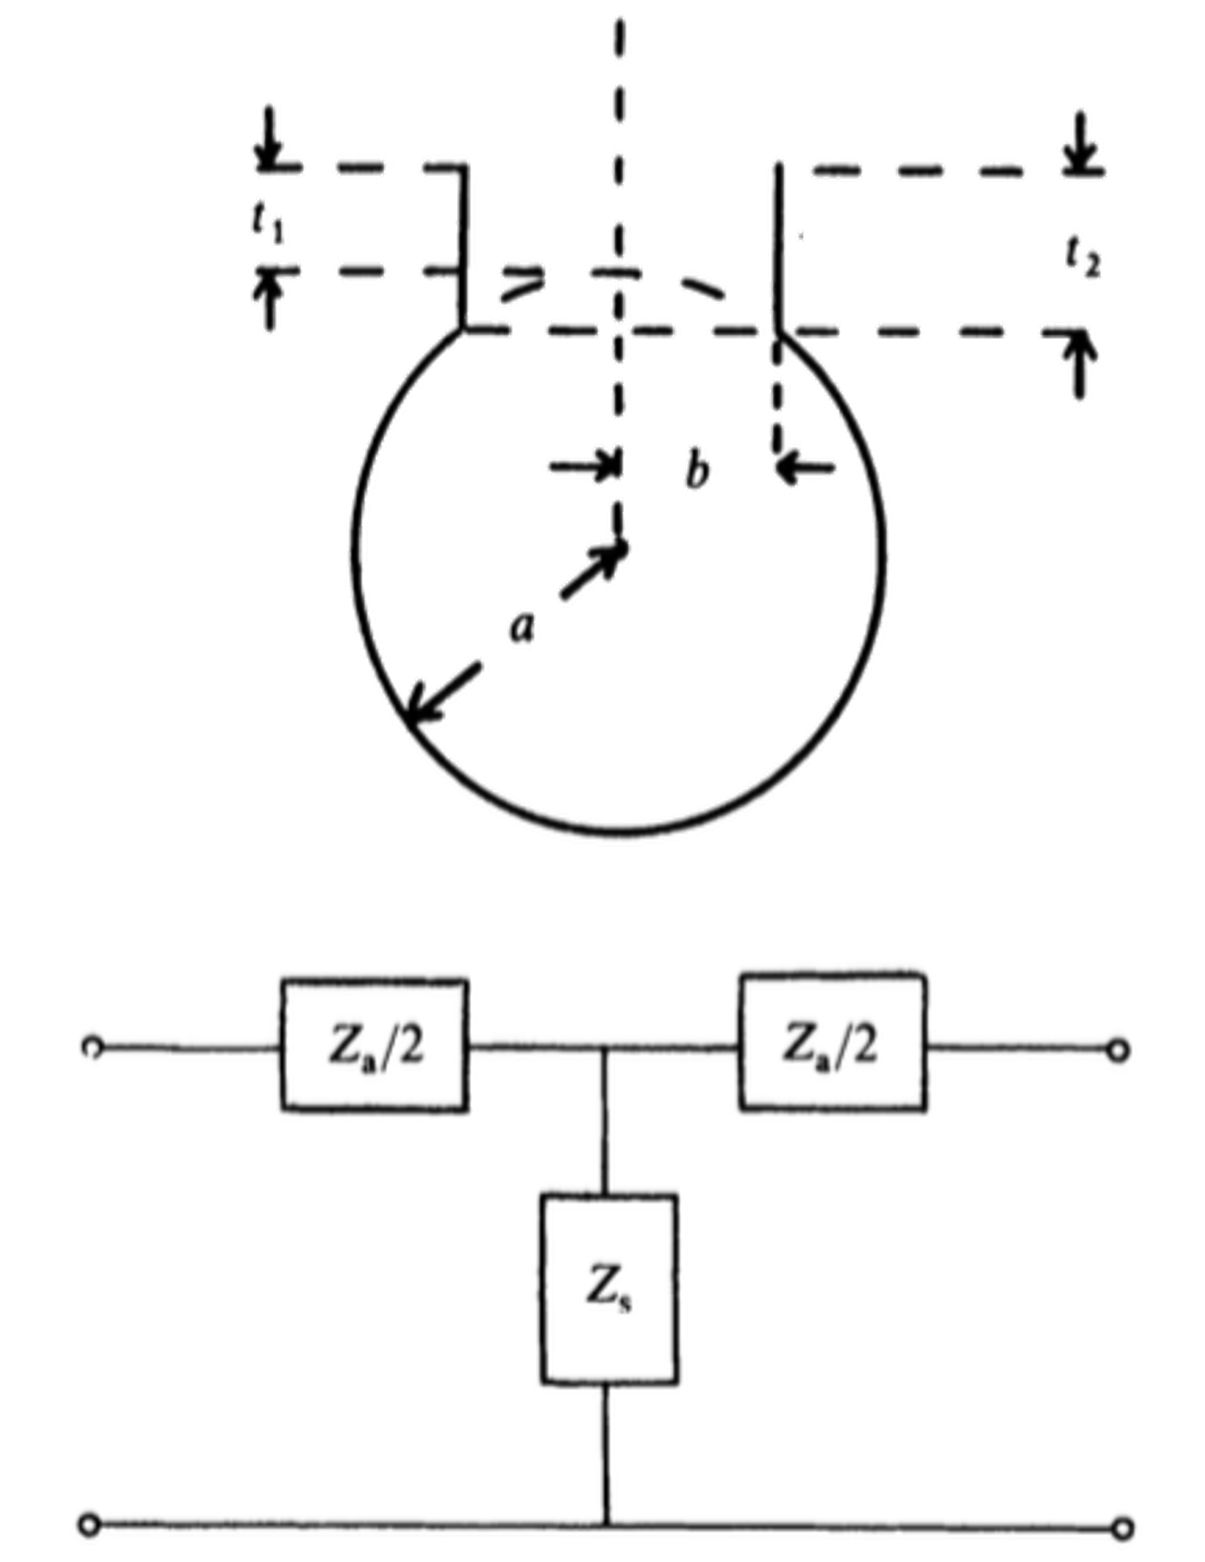
\includegraphics[width=0.7\linewidth]{00_Images/06_chapter/img61.jpg}
\caption{Tone-hole geometry and equivalent network used for impedance computation}
\label{fig:tonehole_model_network}
\end{figure}

\subsection{Impedance Examples}

Measured input-impedance curves illustrate how fingering modifies the resonance pattern.

\paragraph{Clarinet} For a low note and a high note, the frequencies of the fundamental and its harmonics can be marked along the frequency axis. In the higher-note fingering, the first-mode peak is shifted relative to the harmonic grid, indicating that the effective boundary condition created by open holes alters the lowest resonance more strongly than higher ones.

\paragraph{Oboe} For a low note and a high note, the lower impedance peaks exhibit an asymmetric shape, consistent with the influence of a conical bore. In the higher-note fingering, the lower-mode peaks are displaced and reshaped compared to the low-note case.

\section{Sound Radiation}

\subsection{Cutoff Frequency}

The cutoff frequency is the frequency above which sound is radiated freely to the environment without being reflected back into the bore. Above cutoff, the impedance is well coupled to the air characteristic impedance, so pronounced resonances are no longer expected in the radiated spectrum. This aspect contributes strongly to the overall timbre of the instrument. In woodwinds, the cutoff frequency is mostly caused by the presence of finger holes and effectively sets the frequency range over which the instrument behaves as a strongly resonant system. For a pipe of diameter \( 2a \), with holes of diameter \( 2b \) and acoustic length \( l \), separated by \( 2s \), an approximate estimate is
\[
f_c \approx 0.11c\left(\frac{b}{a}\right)\sqrt{\frac{1}{sl}}
\]

\subsection{Sound Radiation Below the Cutoff Frequency}

Sound can radiate from open holes, and the presence of multiple open finger holes makes the radiation pattern complex. The open holes behave like an array of point sources. Below cutoff, several open tone holes can radiate simultaneously; when their phases are similar (typical in the low register), interference leads to a directional pattern that is not purely isotropic, often reduced on-axis and stronger off-axis.

\subsection{Sound Radiation Above the Cutoff Frequency}

Above cutoff, radiation from holes and bell combines. Phase differences between sources produce frequency-dependent lobes and nulls; higher harmonics tend to be more directional, and in practice room reflections partially average these effects.

\subsection{Acoustic Efficiency}

The acoustic output of most woodwind instruments is about \SI{1}{\milli\watt}, corresponding to roughly \SI{80}{\decibel} SPL at \SI{1}{\meter}. The player generates a much greater acoustic pressure than that, on the order of \SIrange{3}{5}{\kilo\pascal}, corresponding to \SIrange{0.3}{0.5}{\watt}. The acoustic efficiency is therefore about \SI{1}{\percent}. The remaining power is mostly absorbed by the reed valve and dissipated by viscous and thermal losses in the pipe.

\subsection{Spectrum Envelope of Reed-Driven Instruments}

The reed strongly influences the radiated sound and can vary greatly with internal nonlinearities, blowing pressure, and playing technique. Tube resonances shape the reed excitation up to the cutoff frequency. Above cutoff, the spectrum exhibits an approximately constant decaying slope of about \SI{-12}{\decibel} for a beating reed and about \SI{-18}{\decibel} for a non-beating reed. An example of how the radiated waveform and spectrum can change with pitch is shown in figure \ref{fig:clarinet_waveform_spectra_example}.

\begin{figure}[!htb]
\centering
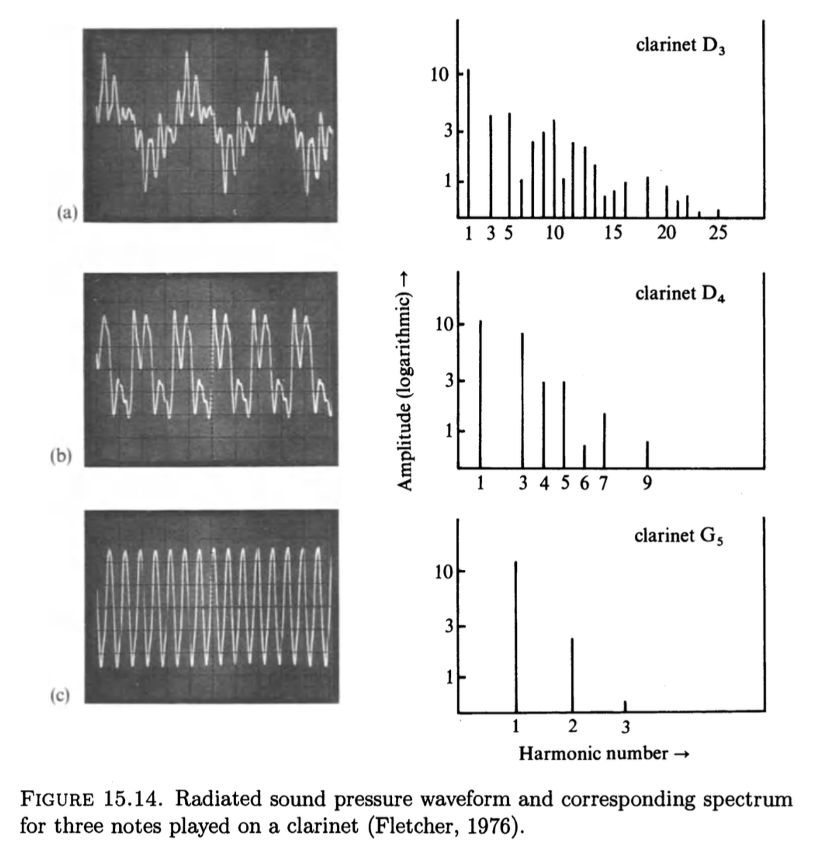
\includegraphics[width=0.7\linewidth]{00_Images/06_chapter/img93.jpg}
\caption{Example of reed-driven waveform and harmonic spectrum across different notes (clarinet)}
\label{fig:clarinet_waveform_spectra_example}
\end{figure}

\section{Woodwind Instrument Overview}

This section summarizes a few representative woodwinds by linking bore geometry, reed type, register mechanism, and spectral features. 

\subsection{Clarinet}

The clarinet is characterized by a cylindrical bore and a single reed. Register changes are achieved through dedicated keys, enabling a wide pitch range: about three octaves organized into two main registers, plus an additional register covering part of the next upper octave. Radiated-pressure waveforms and spectra illustrate how the harmonic content changes across notes, with the low register showing a rich harmonic structure and higher notes exhibiting a different distribution of partials. Representative harmonic spectra for a low and a high clarinet note are shown in figure \ref{fig:clarinet_harmonics_low_high}.

\begin{figure}[!htb]
\centering
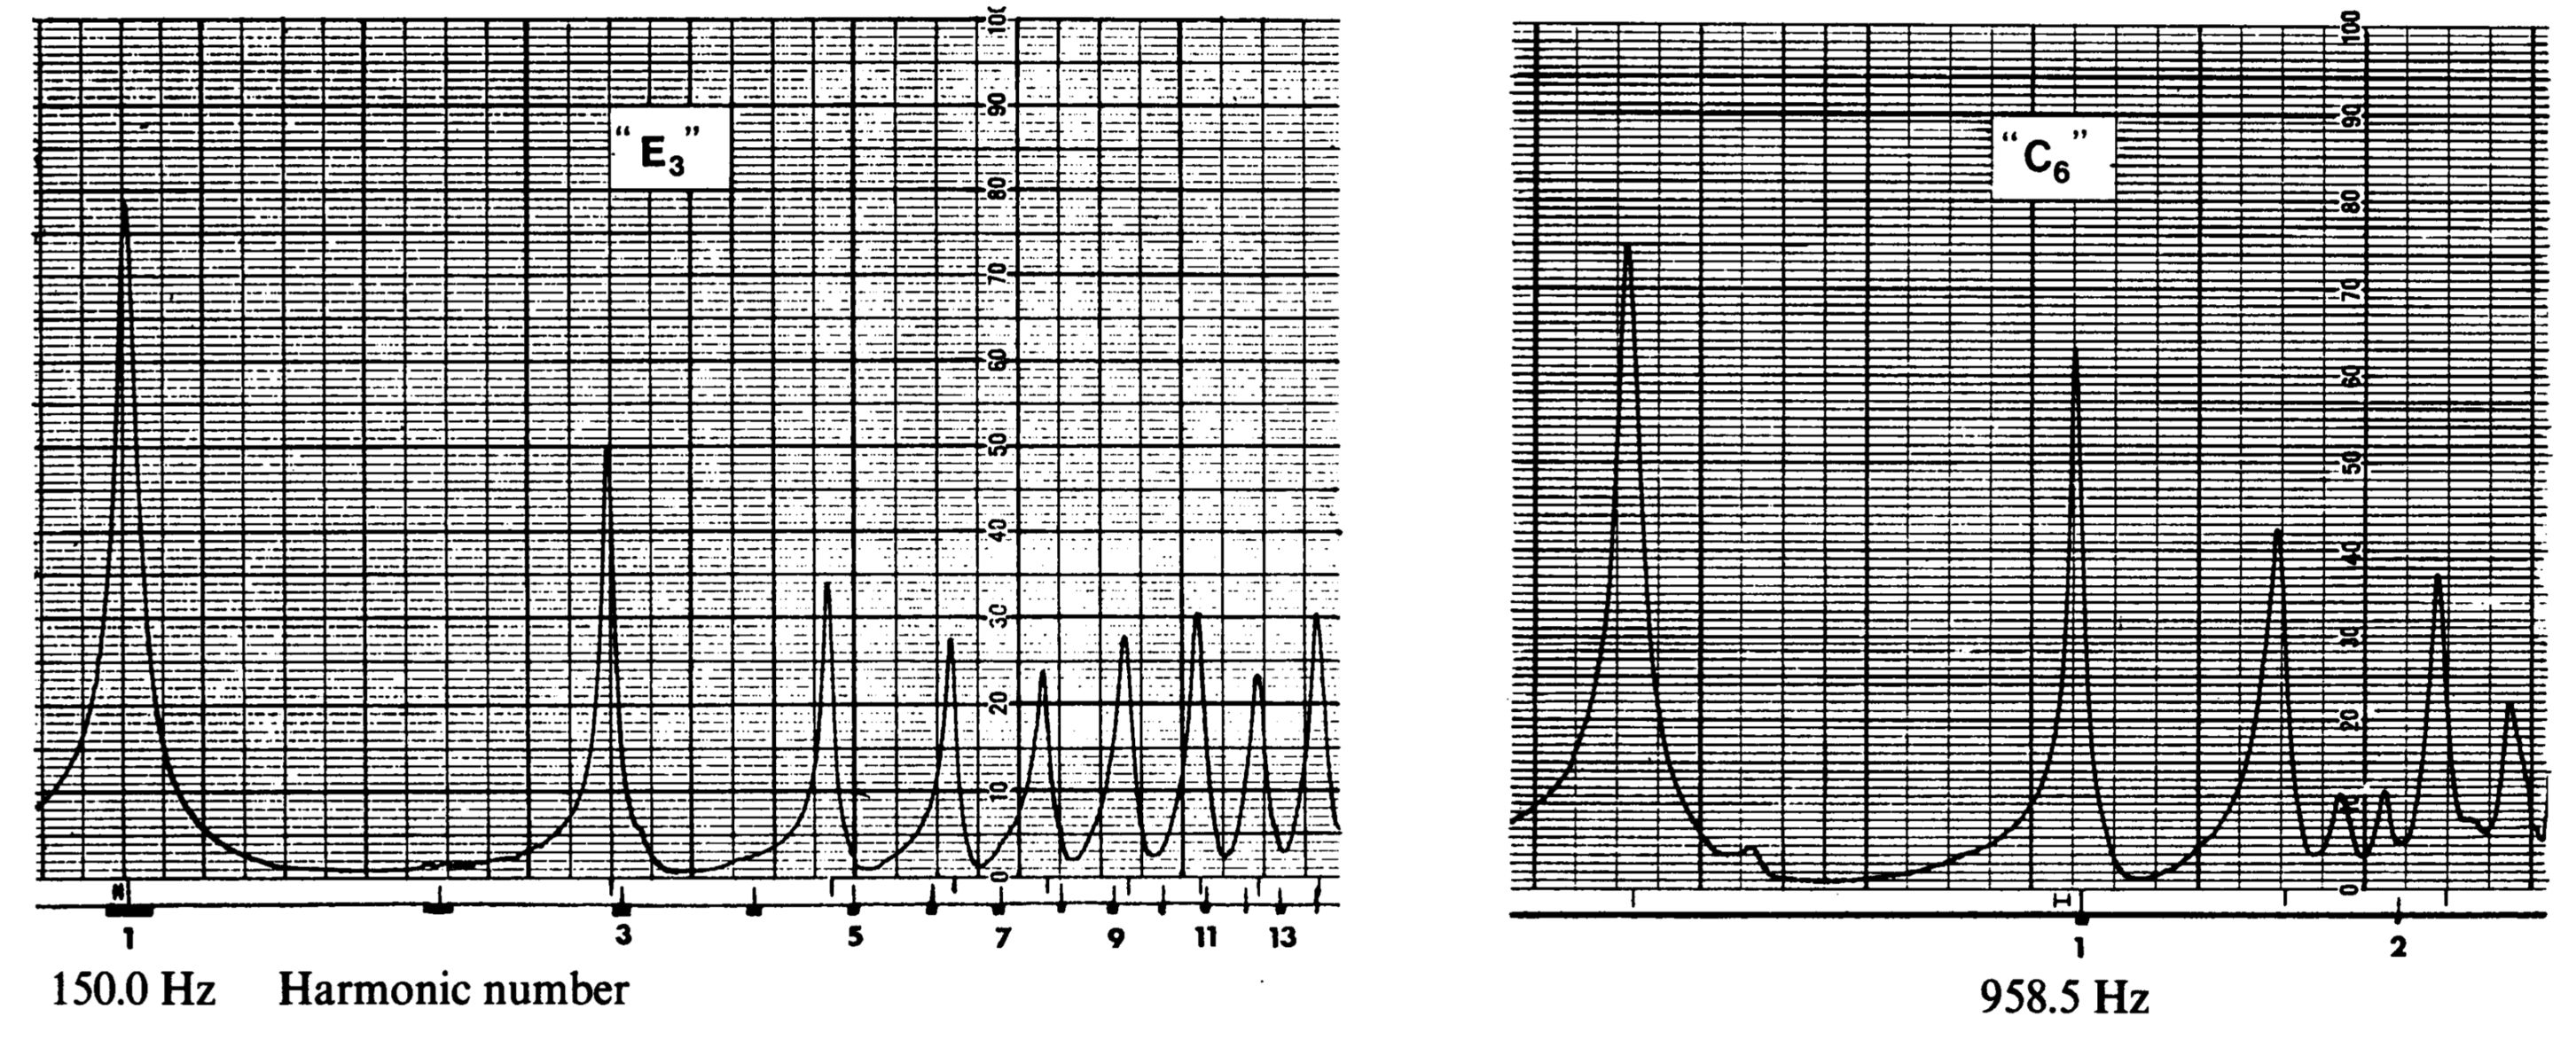
\includegraphics[width=0.7\linewidth]{00_Images/06_chapter/img68.jpg}
\caption{Clarinet harmonic spectra in the low register versus a higher note}
\label{fig:clarinet_harmonics_low_high}
\end{figure}

\subsection{Oboe}

The oboe has approximately the same overall length as the clarinet, but it uses a double reed and a conical bore. A complex keywork allows a large chromatic extension across registers. The conical shape makes the lowest note nearly an octave higher than the clarinet’s lowest note. A relevant playing feature is that the reed always beats, which limits the amount of tone-color variation between soft and loud dynamics compared with non-beating regimes. In spectral terms, lower notes show a strong harmonic spectrum with a comparatively high level of upper harmonics, producing a brighter timbre than the clarinet. The input-impedance peaks and the radiated spectrum initially show peaks rising with frequency, while beyond cutoff the spectrum decreases with a slope of about \SI{-12}{\decibel} per octave, consistent with a beating reed. Representative harmonic spectra for a low and a high oboe note are shown in figure \ref{fig:oboe_harmonics_low_high}.

\begin{figure}[!htb]
\centering
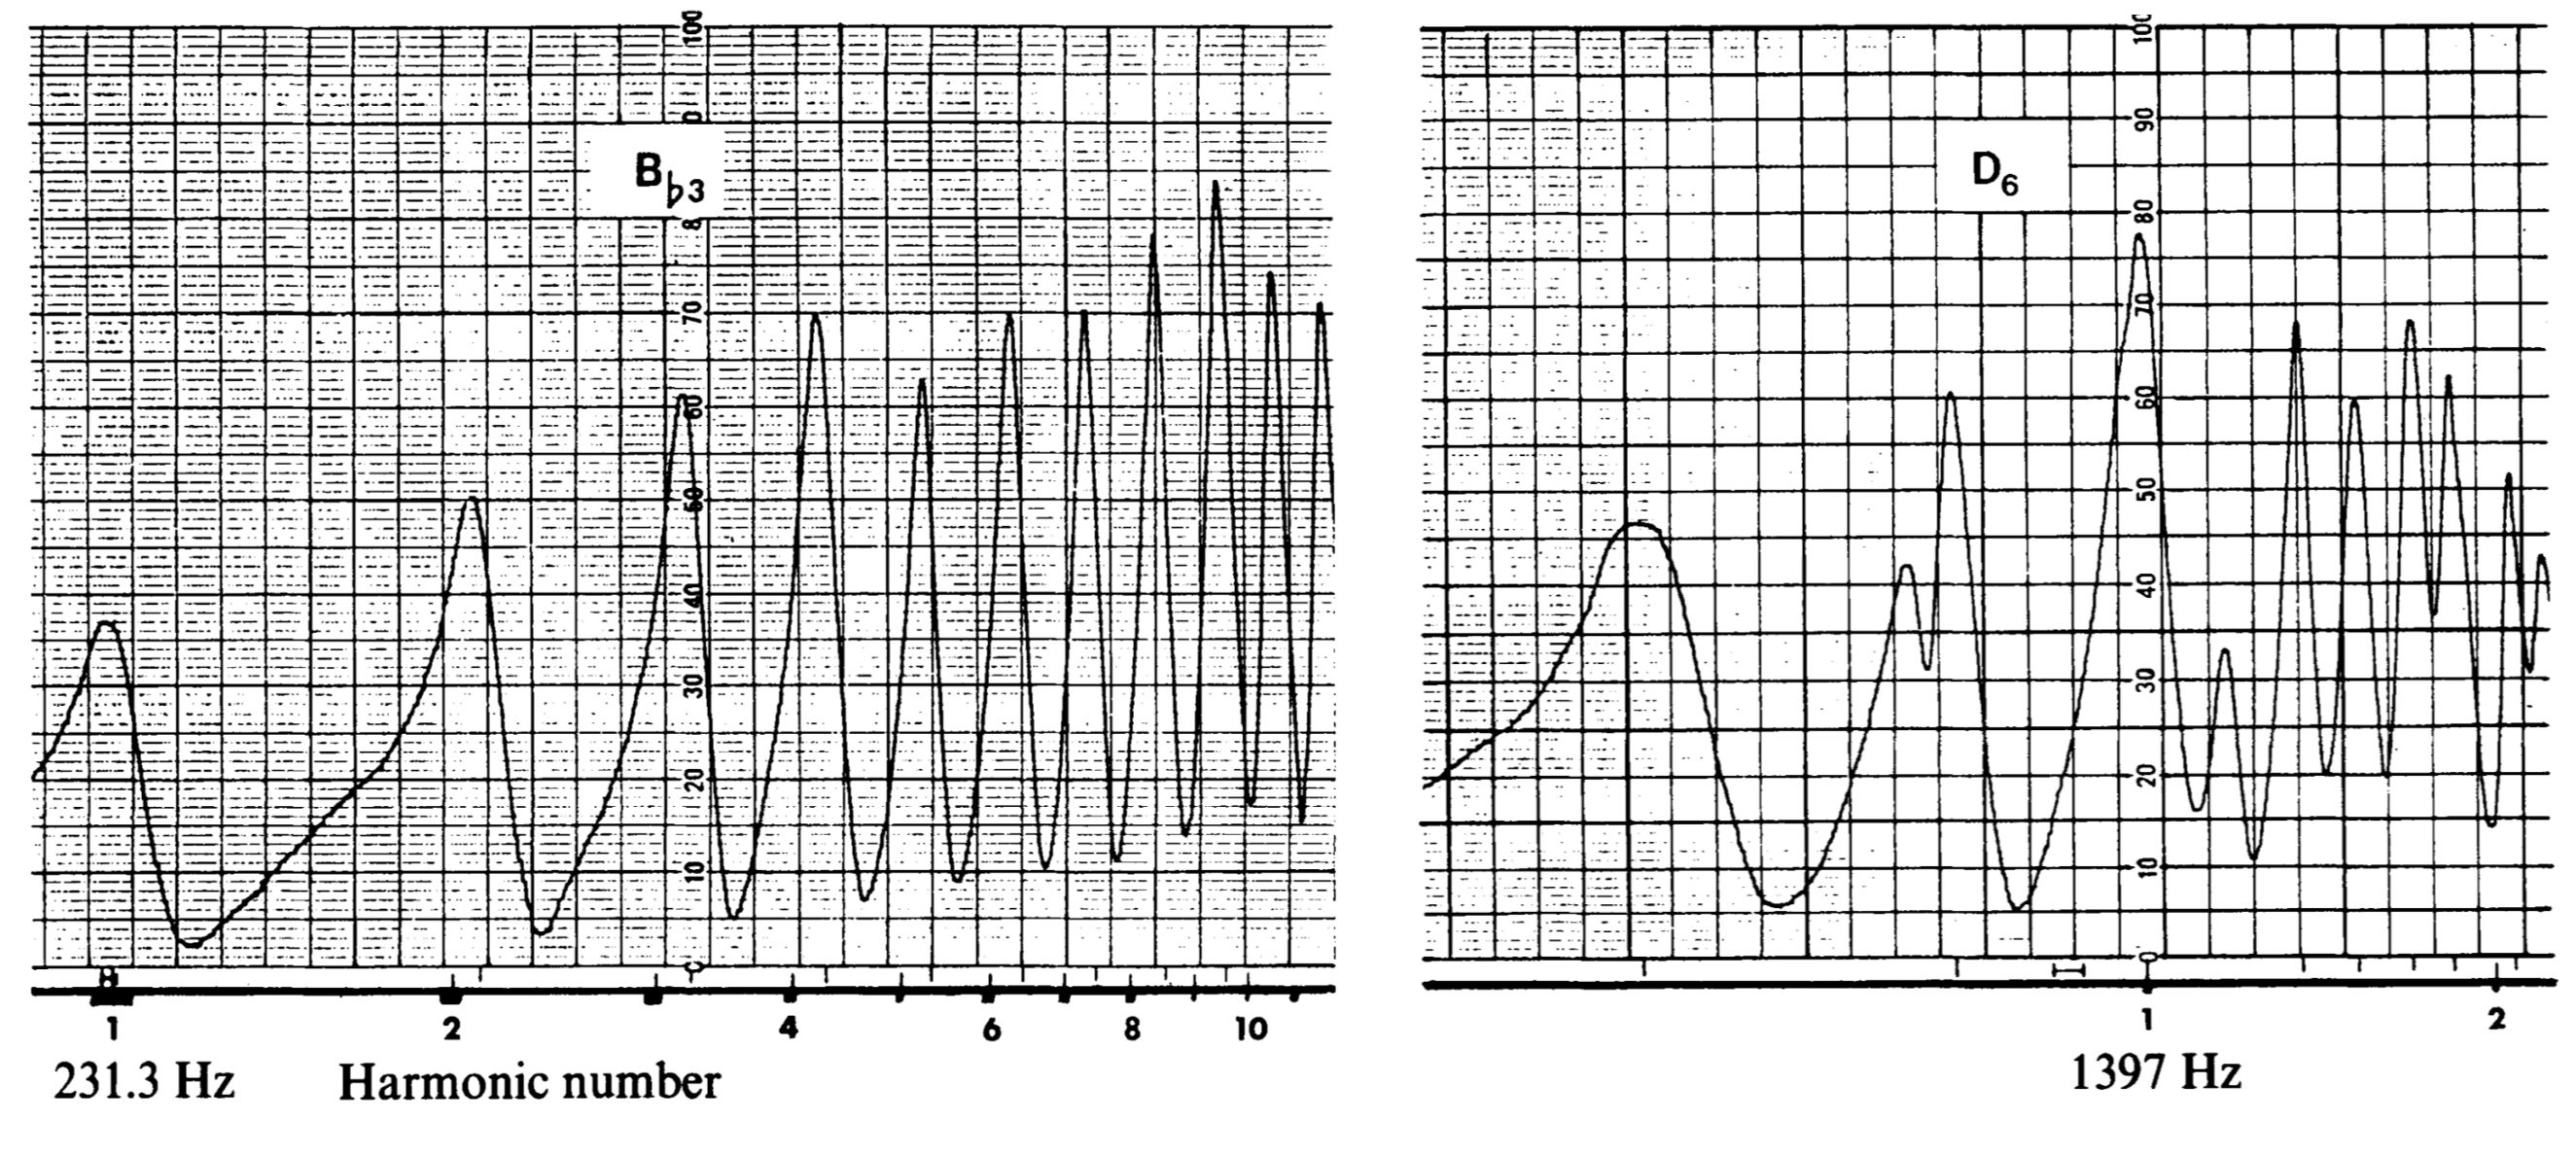
\includegraphics[width=0.7\linewidth]{00_Images/06_chapter/img74.jpg}
\caption{Oboe harmonic spectra in the low register versus a higher note}
\label{fig:oboe_harmonics_low_high}
\end{figure}

\paragraph{Bassoon} The bassoon is also a conical, double-reed instrument. To reach low notes, the tube is folded to obtain a total length of about \SI{2.6}{\meter}. Low notes can have a weak fundamental component because of the tube diameter. The tone is typically mellow and relatively poor in harmonics, which is associated with a low cutoff frequency in the range \SIrange{300}{600}{\hertz}. As for the oboe, the reed always beats, contributing to a limited tone-color change between soft and loud playing. 

\subsection{Saxophone}

The saxophone was designed by Adolphe Sax in the nineteenth century, with characteristics intentionally engineered rather than emerging from a long evolutionary process. It combines a wide conical bore, with flare semiangle around \SI{2}{\degree}, and a clarinet-like single reed. Large tone holes are operated by padded keys. A high cutoff frequency is paired with high radiation efficiency. Reflections are less pronounced than in other woodwinds, so stationary waves are less prominent, and radiation damping is strong for higher partials. A distinctive geometric feature is the sudden truncation of the conical shape at the mouthpiece. To preserve harmonic relationships, the mouthpiece is designed to mimic the acoustic behavior of the cone apex. Consequently, mouthpiece characteristics strongly affect the saxophone spectrum both below and above the cutoff frequency. 
